%!TEX program = lualatex
\documentclass[12pt,letterpaper,fleqn]{article}          % fleqn: align equations left

% File produced by Jeremy West
% This file may be distributed and/or modified:
%   1. under the LaTeX Project Public License and/or
%   2. under the GNU Public License.

% Pretty much required packages for me:
\usepackage{fullpage}                                    % Use the full page
\usepackage{fontspec}
\setmainfont{baskerville}
\usepackage{amsmath}                                     % Math equations, etc.
\usepackage{graphicx}                                    % Enable images (no .eps w/o below option)
\usepackage{epstopdf}                                    % Convert .eps images on the fly
\usepackage{color}                                       % Enables colored text
\definecolor{darkblue}{rgb}{0.0,0.0,0.66}                % Custom color: dark blue
\usepackage[hyperfootnotes=false,bookmarksopen]{hyperref}% Enable hyperlinks, expand menu subtree
\hypersetup{                                             % Custom hyperlink settings
    pdffitwindow=false,                                  % true: window fit to page when opened
    pdfstartview={XYZ null null 1.00},                   % Fits the zoom of the page to 100%
    pdfnewwindow=true,                                   % Links in new window
    colorlinks=true,                                     % false: boxed links; true: colored links
    linkcolor=darkblue,                                  % Color of internal links
    citecolor=darkblue,                                  % Color of links to bibliography
    urlcolor=darkblue  }                                 % Color of external links
\usepackage{booktabs}                                    % For better tables
\newcommand{\ra}[1]{\renewcommand{\arraystretch}{#1}}    % Spacing for tables improved
\renewcommand{\arraystretch}{1.5}                        % Spaces arrays at 1.5x for readability
\usepackage{pdflscape}                                   % Use: \begin{landscape} ... \end{landscape}

% Some "optional" packages that I frequently use:
\usepackage{datetime}                                    % Custom date format for date field
\newdateformat{mydate}{\monthname[\THEMONTH] \THEYEAR}   % Defining month year date format
\usepackage[authoryear]{natbib}                          % Bibliography and citation formating
\usepackage[section]{placeins}                           % Forces floats to stay in section
\usepackage{float}                                       % Used with restylefloat
\restylefloat{figure}                                    % "H" forces a figure to be "exactly here"
\usepackage{textcomp}                                    % Supports many additional symbols
\usepackage{amsthm}                                      % Math theorems, etc.
\usepackage{amsfonts}                                    % Math fonts (e.g. script fonts)
\usepackage{amssymb}                                     % Math symbols such as infinity
\DeclareMathOperator*{\Max}{Max}                         % Better looking max function
\DeclareMathOperator*{\Min}{Min}                         % Better looking min function
\usepackage{subfig}                                      % Enables arrayed images
\usepackage{setspace}                                    % Enables custom margins, doublespacing, etc.
\usepackage{tikz}                                        % Timelines and other drawings
\usetikzlibrary{decorations}                             % Formating for Tikz


\usepackage{color}

\definecolor{mygreen}{rgb}{0,0.6,0}
\definecolor{mygray}{rgb}{0.5,0.5,0.5}
\definecolor{mymauve}{rgb}{0.58,0,0.82}
\definecolor{light-gray}{gray}{0.95}
\usepackage{listings}

\lstdefinestyle{customc}{
backgroundcolor=\color{light-gray},
  belowcaptionskip=1\baselineskip,
  breaklines=true,
  frame=single,
  xleftmargin=\parindent,
  language=C++,
  showstringspaces=false,
  basicstyle=\footnotesize\ttfamily,
  keywordstyle=\bfseries\color{green!40!black},
  %commentstyle=\itshape\color{purple!40!black},
  identifierstyle=\color{blue},
  %stringstyle=\color{orange},
  numberstyle=\tiny\color{mygray},
  numbers=left,                    % where to put the line-numbers; possible values are (none, left, right)
  numbersep=5pt,                   % how far the line-numbers are from the code
  commentstyle=\color{mygreen},
  stringstyle=\color{mymauve},
}

\lstdefinestyle{customasm}{
  belowcaptionskip=1\baselineskip,
  frame=L,
  xleftmargin=\parindent,
  language=[x86masm]Assembler,
  basicstyle=\footnotesize\ttfamily,
  commentstyle=\itshape\color{purple!40!black},
}

\lstset{escapechar=@,style=customc}

\usepackage{titlesec}
\usepackage{lipsum}
\titleformat{\section}
  { \large \normalfont\scshape}{\thesection}{1em}{}
  \titleformat{\subsection}
  { \normalfont\scshape}{\thesection}{1em}{}

  
\newcommand{\horrule}[1]{\rule{\linewidth}{#1}} 	% Horizontal rule

\title{
		%\vspace{-1in} 	
		\usefont{OT1}{bch}{b}{n}
		\normalfont \normalsize \textsc{ \fontspec{Zapfino} King Abdullah University of Science and Technology} \\ [25pt]
		\horrule{0.5pt} \\[0.4cm]
         \Large Fall 2015 CS 247 Scientific Visualization Assignment 3\\
		\horrule{2pt} \\
}

\author{Gang Liao \hspace{1.05cm} ID: 133267 }

\begin{document}

\maketitle

\onehalfspacing

\section{Glyph visualization}
Some basic matrix transformation in computer graphics, for instance, translation, rotation, scale can be used to draw arrows for vector field visualization.

\begin{lstlisting}
void draw_arrow_head(float head[2], float direct[2])
{
  float M_PI = 3.1415926;
  glPushMatrix();
  glTranslatef(head[0], head[1], 0);
  glRotatef(atan2(direct[1], direct[0]) * 360 / (2 * M_PI), 0, 0, 1);
  glScalef(0.03, 0.03, 1);
  glBegin(GL_TRIANGLES);
  glVertex2f(0, 0);
  glVertex2f(-0.35, 0.12);
  glVertex2f(-0.35, -0.12);
  glEnd();
  glPopMatrix();
}
\end{lstlisting}


	
\begin{figure}[!htb]
\centering
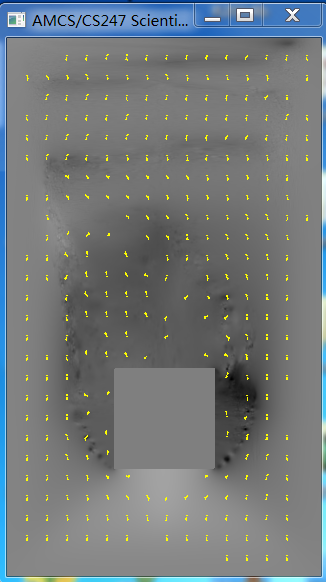
\includegraphics[scale=0.70]{4}
\end{figure}

\section{Streamlines}

\begin{figure}[!htb]
\centering
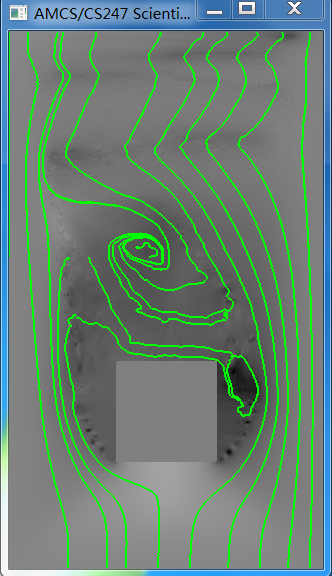
\includegraphics[scale=0.70]{1}
\end{figure}

\begin{figure}[!htb]
\centering
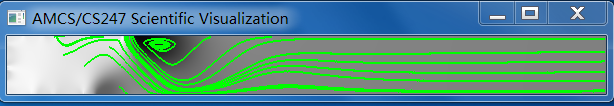
\includegraphics[scale=0.70]{2}
\end{figure}

\begin{figure}[!htb]
\centering
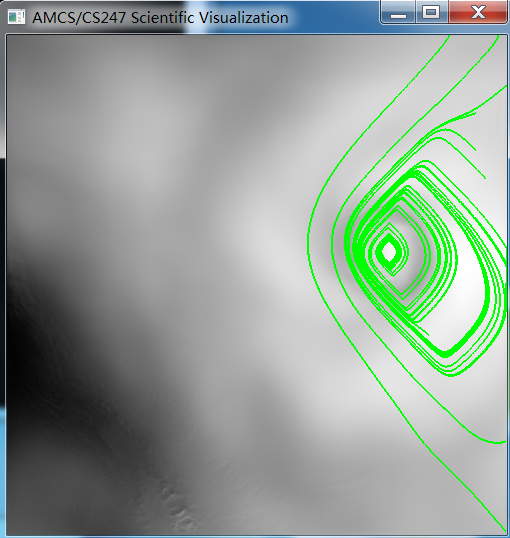
\includegraphics[scale=0.70]{3}
\end{figure}

\section{Pathlines}
\begin{figure}[!htb]
\centering
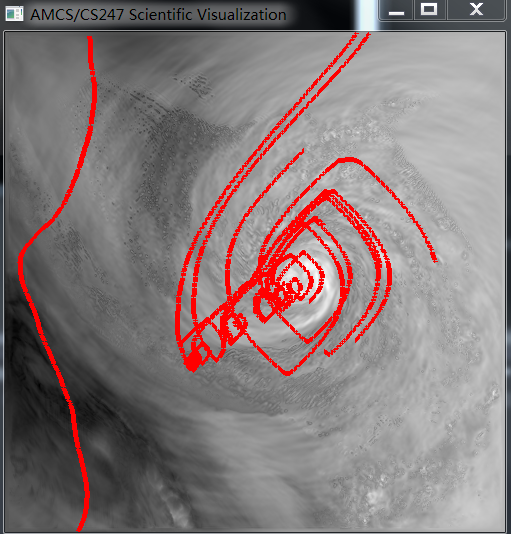
\includegraphics[scale=0.70]{5}
\end{figure}

\section{Bonus}

\subsection*{1. multiple streamline seeds}
for horizontal rake:
\begin{lstlisting}
stream_pos.clear();
    if (isStreamline == true)
    {
      for (int i = 0; i < vol_dim[0]; i+=samp_rate)
      {
        stream_pos.push_back(i);
        stream_pos.push_back(seed_y);
      }
    }
\end{lstlisting}

for vertical rake:
\begin{lstlisting}
stream_pos.clear();
    if (isStreamline == true)
    {
      for (int i = 0; i < vol_dim[1]; i += samp_rate)
      {
        stream_pos.push_back(seed_x);
        stream_pos.push_back(i);
      }
    }
\end{lstlisting}

\subsection*{2. scalar field images}

\begin{lstlisting}
case 's':
    current_scalar_field = (current_scalar_field + 1) % num_scalar_fields;
    DownloadScalarFieldAsTexture();
    fprintf(stderr, "Scalar field changed.\n");
    break;
\end{lstlisting}

\subsection*{3. RK4}
It's very similar to RK2 and easy to implement.

%%%%%%%%%%%%%%%%%%%%%%%%%%%%%%%%%%%%%%%%%%%    REFERENCES
%\clearpage
%\singlespacing
%\bibliographystyle{plainnat}
%\bibliography{filename} % Name of .bib references file
%\clearpage

%\vspace{3cm}

%%%%%%%%%%%%%%%%%%%%%%%%%%%%%%%%%%%%%%%%%%%    TABLES & FIGURES
%\newpage
%\section{Tables and Figures}\label{sec:tables}


%%%%%%%%%%%%%%%%%%%%%%%%%%%%%%%%%%%%%%%%%%%    APPENDIX
%\newpage
%\appendix
%\section{Appendix}\label{sec:appendix}


\end{document}
